\documentclass{article}
\usepackage[utf8]{inputenc}
\usepackage[spanish]{babel}
\usepackage{amsmath}
\usepackage{amsfonts}
\usepackage{amssymb}
\usepackage{graphicx}
\usepackage[left=2cm,right=2cm,top=2cm,bottom=2cm]{geometry}
\usepackage[hidelinks]{hyperref}
\usepackage{listings}

\lstset {
    frame = single, breaklines = true
}

\begin{document}

\begin{titlepage}
\title{\textbf{
    {\Huge Práctica 5: Condiciones de Carrera}\\
    {\Large Seguridad Informática}
}}
\author{
    Pedro Allué Tamargo (758267)
    \and
    Juan José Tambo Tambo (755742)
}
\date{\today}
\clearpage\maketitle
\thispagestyle{empty}
\tableofcontents
\end{titlepage}

\section{Programa vulnerable}

Se ha implementado el programa \textit{Compra.java} (Código \ref{list:compraVulnerable}) para poder explotar la vulnerabilidad. Se puede observar que el programa sigue el comportamiento esperado pero que existe una variable (\texttt{saldoActual}) que almacena el saldo al inicio. Esta variable será clave para explotar la vulnerabilidad de condiciones de carrera.\\


\section{Explotación de la vulnerabilidad}

\subsection{¿Cúales son los recursos compartidos? ¿Quién los comparte? ¿Cúal es la ventana temporal de la vulnerabilidad?}
\begin{itemize}
    \item Los recursos compartidos son los ficheros: \textit{carrito.txt} y \textit{cuenta.txt}
    \item Estos recursos son compartidos por las distintas instancias de \textit{Cuenta} y \textit{Carrito}.
    \item La ventana temporal es el tiempo en el que un recurso puede ser modificado por otra secuencia de código que se ejecuta concurrentemente. Por lo tanto, en el código implementado la ventana temporal sería cualquier ejecución mientras haya un programa esperando la entrada de información por parte del usuario. En este caso el programa esperando la entrada del usuario habrá almacenado el saldo disponible cuando comenzó su ejecución. La variable culpable de esta vulnerabilidad es \texttt{saldoActual} (línea 20).\\
    No obstante, si no hubiese existido esta variable se hubiera podido explotar la vulnerabilidad con una ventana temporal más reducida en el momento de la escritura del saldo en el fichero \textit{cuenta.txt}. Esto es así ya que al introducir un retraso entre la lectura del saldo y su escritura en el fichero existe la posibilidad de que otro programa lea el saldo no actualizado.
\end{itemize}

Para explotar la vulnerabilidad se han ejecutado concurrentemente dos instancias de \texttt{Compra.java} (Figura \ref{fig:p1_1}). Al inicio ambos programas almacenan el saldo actual proporcionado por la \textit{API} de \textit{Cuenta}. Ahora, ambos programas pedirán la compra de un coche. Al ejecutarse de manera concurrente e independientemente del orden (ya que ambos han almacenado el saldo al principio de la ejecución) se comprarán dos coches. Se puede observar el saldo resultante y el carro de la compra en la Figura \ref{fig:p1_2}.

\begin{figure}[h!]
    \centering
    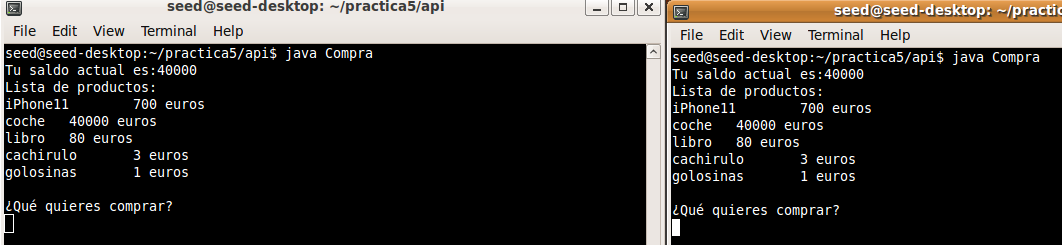
\includegraphics[scale=0.65]{images/p1_1.png}
    \caption{Captura de pantalla de la ejecución concurrente de dos instancias de \texttt{Compra.java}}
    \label{fig:p1_1}
\end{figure}

\begin{figure}[h!]
    \centering
    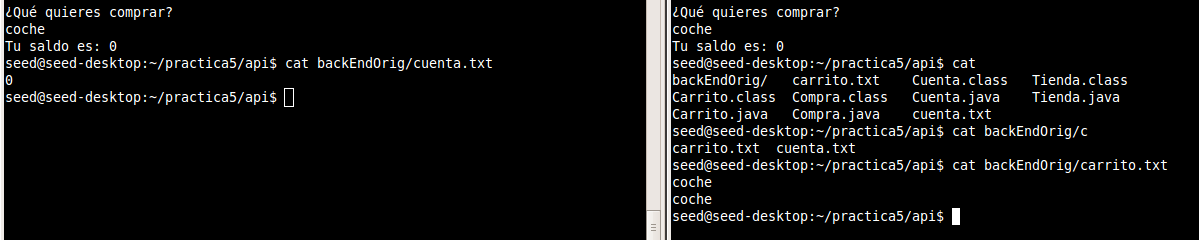
\includegraphics[scale=0.58]{images/p1_2.png}
    \caption{Captura de pantalla de los resultados de ejecución concurrente de dos instancias de \texttt{Compra.java}}
    \label{fig:p1_2}
\end{figure}

\section{Corrección de las \textit{API}}

\subsection{Creación del método \texttt{sacarDinero} de \textit{Cuenta.java}}

Para impedir la vulnerabilidad de condición de carrera se va a implementar una función en la clase \texttt{Cuenta} que combine el comportamiento de \texttt{obtenerSaldo} y el de \texttt{establecerSaldo}. Este cambio reducirá la ventana de temporal pero no impedirá que existan entrelazados que permitan la existencia de condiciones de carrera.\\
Para resolver esto se han utilizado clases \textit{Java} para permitir el acceso en exclusión mutua al fichero \textit{cuenta.txt}. Los mecanismos utilizados han sido \texttt{FileChannel} para obtener un canal por el cual manipular el fichero y bloquearlo, y \texttt{FileLock} para obtener el bloqueo proporcionado por el canal. Se utilizará el método \texttt{lock()} de la clase \texttt{FileChannel} que tiene comportamiento bloqueante para obtener el \texttt{lock} sobre el fichero \textit{cuenta.java}.\\
El código de esta \textit{API} se puede encontrar en el Código \ref{list:sacarDinero}.\\


\subsection{¿Hay otras \textit{API} vulnerables a la condición de carrera?}

Otra de las \textit{APIs} vulnerables sería \textit{Carrito.java}, ya que podría darse el caso de que dos procesos intentasen escribir (método \texttt{writeBytes} de la clase \texttt{RandomAccessFile}) al mismo tiempo y en la misma parte del fichero el producto comprado. Para evitarlo, se podría utilizar una solución como la comentada en el apartado anterior (\textit{FileLock}) para evitar la posibilidad de que dos procesos se solapen en la escritura del fichero.\\


\subsection{Implementar una versión de \textit{CompraSegura.java}}

Se ha implementado una versión segura de \texttt{Compra.java} que reduce la ventana temporal de la vulnerabilidad de condición de carrera y además utiliza la función \texttt{sacarDinero} comentada anteriormente para evitar fallos debido a una escritura después de lectura en el fichero \textit{cuenta.txt}. Si se intenta replicar la ejecución de la Figura \ref{fig:p1_1} se obtiene que una de las dos instancias informa de que el saldo no es suficiente. Si se observan los ficheros \textit{cuenta.txt} y \textit{carrito.txt} se comprobará que no hay saldo en la cuenta (\textit{saldo = 0}) y que en el carrito solo se ha añadido el elemento \textit{coche} una vez. Este comportamiento se puede observar en la Figura \ref{fig:comportamientoCompraSegura}.\\
El código de esta clase se puede encontrar en el Código \ref{list:compraSegura}.\\

\begin{figure}[h!]
    \centering
    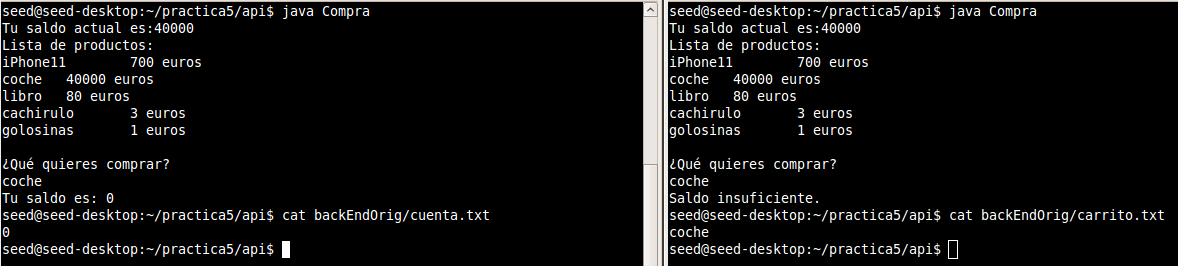
\includegraphics[scale=0.56]{images/p3.png}
    \caption{Captura de pantalla del comportamiento de \texttt{CompraSegura.java}}
    \label{fig:comportamientoCompraSegura}
\end{figure}


\newpage
\section{Anexo 1: Códigos}

\subsection{Código vulnerable \textit{Compra.java}}
\lstinputlisting[label={list:compraVulnerable}, language=Java]{listings/Compra.java}

\subsection{Código de la implementación de \texttt{sacarDinero()}}
\lstinputlisting[label={list:sacarDinero}, linerange={56-73}, language=Java]{listings/Cuenta.java}

\newpage
\subsection{Código seguro \texttt{compraSegura}}
\lstinputlisting[label={list:compraSegura},  language=Java]{listings/CompraSegura.java}

\end{document}
